\documentclass[11pt]{article}

\usepackage{graphicx}

% Enable references to labels in the notes
\usepackage{xr-hyper}
\externaldocument{p328_notes}
\usepackage{hyperref}

% Sans fonts
\usepackage{sfmath}
\renewcommand{\familydefault}{\sfdefault}

\newcommand{\COURSE}{PHYS328W}
\newcommand{\LABNUM}{4}
\newcommand{\TITLE}{An RLC Filter}
\markright{\COURSE~Lab \LABNUM\ : \TITLE}

\setlength{\textwidth} {6.5 true in}
\setlength{\textheight}{9 true in}
\setlength{\hoffset}   {-0.75 true in}
\setlength{\voffset}   {-0.75 true in}
\setlength{\parindent} {12 pt}
\pagestyle{myheadings}

\begin{document}

\thispagestyle{empty}

\section*{\COURSE\ Lab \LABNUM\ : \TITLE}

\subsection*{Calculations}

\begin{figure}[h]
\centering
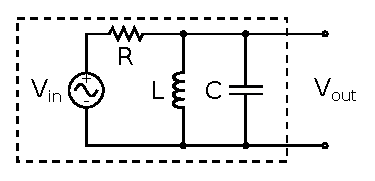
\includegraphics{rlcparallel.eps}
\caption{A Parallel RLC voltage divider.}
\label{fig:rlcparallel}
\end{figure}

In your log book, ...

\begin{enumerate}
\item Derive expressions for the gain, phase angle, resonant
  frequency, and 3~dB points of the circuit. You may find
  Section~\ref{sec:AC} of the notes helpful.

\item Pick out an inductor in the 100-1000~$\mu$H range, and then find
  a capacitor and resistor you predict will give a resonant frequency
  close to 1~MHz and a band width (the difference between the two 3~dB
  points) of no more than 10~kHz.
\end{enumerate}

\subsection*{Simulation}

Simulate your design, and check that it meets the specifications. Use
a linear AC sweep analysis in the region of the resonant frequency
(500~kHz - 1.5~MHz), and be sure to include lots of points (1000) so
that the point spacing is much smaller than the width of the resonance. 
You can use the 
\includegraphics{PSpiceAD_DefineMeasurement.png} button to
set up a band width calculation (\verb+Bandwidth_Bandpass_3dB()+).

\subsection*{Experiment}

\begin{enumerate}
\item Check that your oscilloscope probes are compensated.

\item Build your circuit, and make measurements to produce gain
  vs. frequency and phase angle vs. frequency plots.

\item Measure the 3~dB points and determine the band width.
\end{enumerate}

\subsection*{Product}

Upload to Canvas ...
\begin{itemize}
\item A scan or image of your derivations of expressions for the gain,
  phase angle, resonant frequency, and 3~dB points of the circuit. 

\item The PDF of a brief \LaTeX\ report in which you discuss the
  degree of agreement between theoretical predictions, simulation, and
  measurements. Include as figures plots of your measured gain
  vs. frequency and phase angle vs. frequency plots compared with
  theoretical curves. Comment on any discrepancies you observed
  between theoretical predictions, simulations, and measurements.
\end{itemize}

\end{document}
